\chapter{A szabályozás áttekintése}\label{chap:control}

A hasonló feladatokra leggyakrabban modell-prediktív (MPC) szabályozást használnak \cite{AFRAM2014343}. Ehhez szükség van a szakasz modelljére, ami alapján a szabályzó szimulálhatja a szakasz kimenetét. Az MPC egy beavatkozójel kiadása előtt több mintavételi perióduson, egy predikciós horizonton keresztül fut le, minden lehetséges  beavatkozójel-sorozatra a kimenetet szimulálva.
%A csúszóablak miatt receding horizon control
Ezen sorozatok közül a legjobbat kiválasztja és egy lépést végrehajt. Ezután a szimuláció újrakezdődik. A végrehajtott, adott horizonton optimális beavatkozójelet egy költségfüggvény minimalizálásával kapja. A költségfüggvényben különböző eltéréseknek vagy abszolútértékeknek különböző súlya lehet.

A szabályozás tehát képes egy horizontig előre tekinteni, és azon belüli optimális beavatkozást végrehajtani. (Az angol nyelvű irodalom erre \textit{receding horizon} névvel hivatkozik.) Az optimalizációt minden mintavételkor végrehajtja, így képes korrigálni, ha a jósolt kimenet és a tényleges kimenet eltérő.

A stabilitás a beavatkozó jelek és a zavarjel (külső hőmérséklet) korlátosságából fakad. Ezeket is be lehet állítani a szabályzón, így az MPC a szelepekre csak 0 és 1 közötti beavatkozó jelet fog kiadni.

\vspace{6pt}



\subsection{Fejlesztési lehetőségek a szabályozással kapcsolatban}
	
Épületautomatikai rendszerek használatával, például az iContrALL intelligens otthon rendszerével a fellépő zavarásokat (emberek jelenléte, napsütés, szél) mérhetjük. A szabályozás a zavarások hatásmechanizmusának ismeretében jobb zavarelnyomást tud elérni, sőt az integrációval további beavatkozók is használhatók (például árnyékolástechnikai eszközök).

\pagebreak

\chapter{Önálló labor munka}



{\Large \underline{Motiváció}} \cite{Opticontrol-II}A szakdolgozatban elkezdett munkát folytatva a cél az ottani MPC szabályozás finomhangolása, továbbfejlesztése volt. 
A felállított Simulink modellen a szabályozást kvantitatíven vizsgáltam meg, koncentrálva a költségek és a komfort közötti egyensúlyra. 


{\large \underline{A modell}}
A korábbiakban használt \textit{fűtési rendszer modelljét} nem változtattam meg, viszont a modellből kivezetve mértem a pillanatnyi hőleadást. Így megkaptam a hőmennyiségeket, amik a beavatkozás forintosított költségével arányosak. 


\begin{figure}[H]
	\centering
	% trim={<left> <lower> <right> <upper>}
	%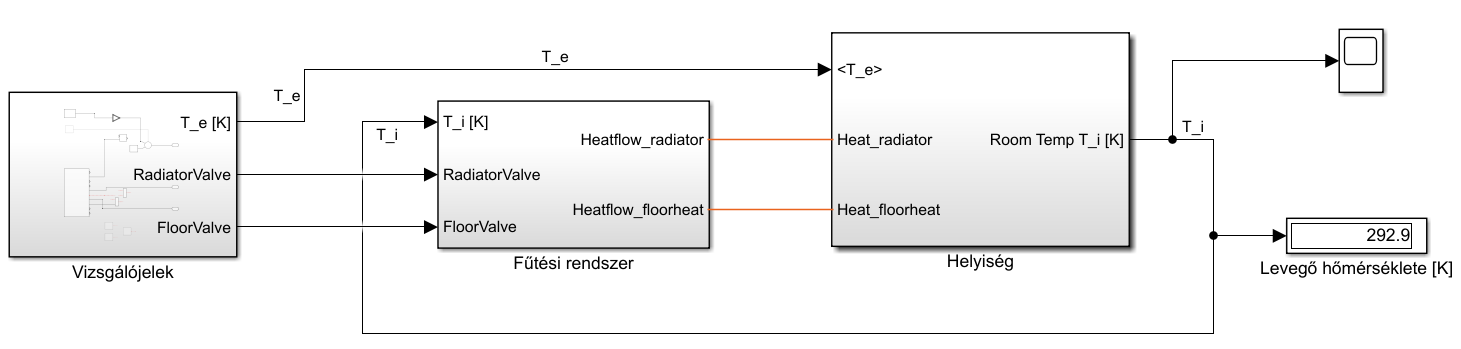
\includegraphics[trim=0 0 0 0, clip,width=\textwidth]{figures/simulink-network-minimalist-layout2}
	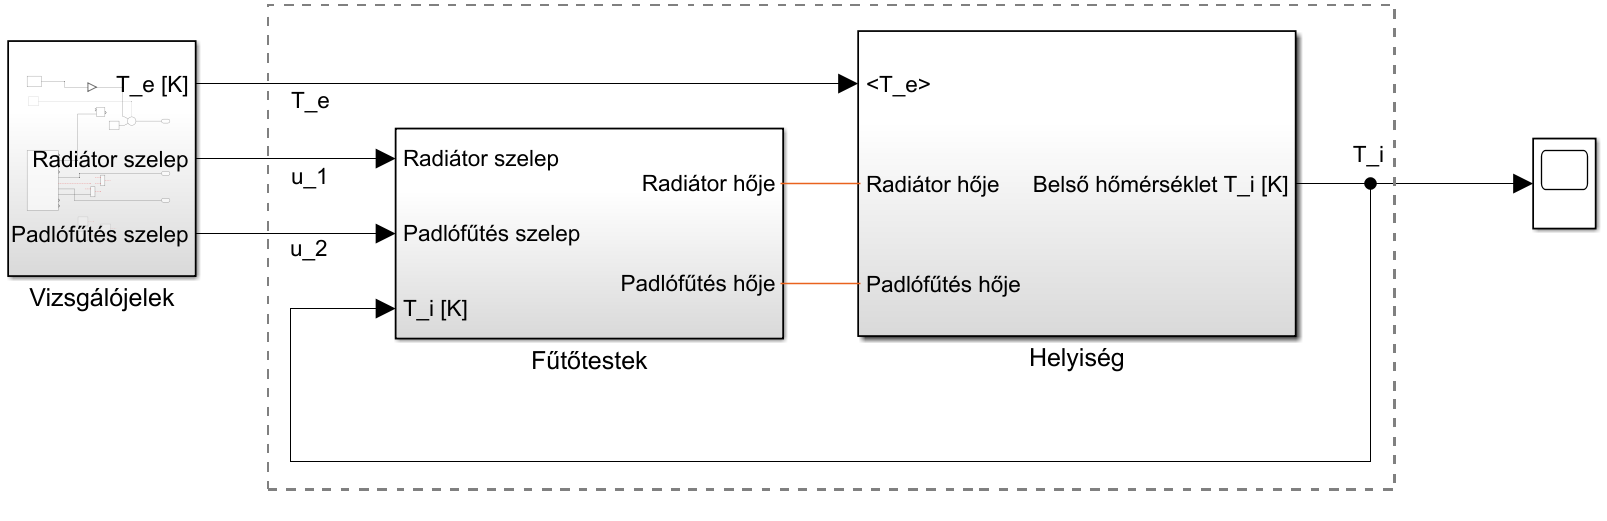
\includegraphics[trim=0 0 0 0, clip,width=\textwidth]{figures/simulink-network-minimalist-layout}
	\caption{Fűtési rendszer modellje - fűtőtest és helyiség}
	\label{fig:Simulink-minimalist}
\end{figure}

Adott környezeti hőmérséklet és belső hőmérséklet (alapjel) mellett ez az energiamennyiég azonos volt, mivel a helyiség hőveszteségei csak ennek különbségétől függnek. Az energiamegtakarítást tehát nem itt kell keresni, hanem a primer energia felhasználásánál. Ennek okai a következők:

Az alacsony hőmérsékletű (sugárzó) fűtések, pl. a padlófűtés használata gazdaságosabb lehet a hagyományos radiátoros fűtéseknél a megújulók használatával. Ugyanannyi leadott energia így olcsóbb ilyen rendszerekkel\footnote{Sugárzó fűtésekkel kevesebb primer energia szükséges a jobb hatásfok, kisebb veszteségek miatt.}, emellett pedig jobb hőérzetet biztosítanak.

A modellben a kétféle fűtőtesthez két külön beavatkozó jel tartozik, mely a két szelep kinyitásának mértéke. A beavatkozók dinamikája is eltér, a prediktív irányítás ezt figyelembe véve tud egy egyensúlyt találni.

A csúcsterhelés csökkentése számos előnnyel jár. Szakaszos üzem helyett folyamatos teljesítményigény esetén a megújuló források előnyösebben hasznosíthatók. 

\section{MPC áttekintés}

A modell-prediktív szabályozást alapjaiban a szakdolgozatomban mutattam be. A szabályozó, illetve a zárt szabályozási kör blokkvázlata és a rövidítések magyarázata szerepel az alábbiakban.
\cite{MPCtoolboxGuide} alapján


\begin{figure}[h]
	\centering
	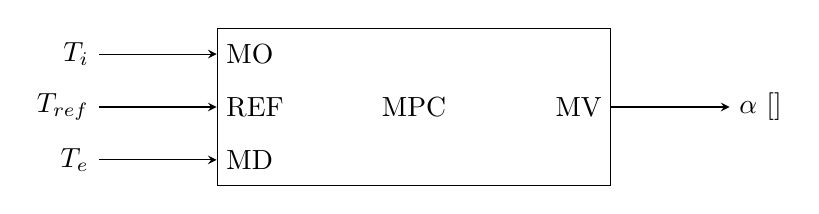
\begin{tikzpicture}[>=stealth]
	% Controller
	% ----------
	\node[draw,rectangle, minimum height=2cm,minimum width=5cm,
		  %label={[xshift=1.0cm, yshift=0.3cm]Label},
		  %label={[xshift=-4.1cm, yshift=-0.7cm]Label},
		  ]
		  (MPC) at (2.3,2.5) {\parbox{2cm}{\centering MPC}};	
	
	% az MPC doboz bemenetei
	\draw [<-] (MPC.165) node[right]{MO} -- +(-15mm,0) node[left]{$T_i$};
	\draw [<-] (MPC.180) node[right]{REF} -- +(-15mm,0) node[left]{$T_{ref}$};
	\draw [->] (MPC.0) node[left]{MV} -- +(15mm,0) node[right]{$\alpha$ [\si{\percent}]};
	\draw [<-] (MPC.195) node[right]{MD} -- +(-15mm,0) node[left]{$T_e$};
	
	\end{tikzpicture}

	\caption{Az MPC be- és kimenetei}
	\label{fig_mpcinout}
\end{figure}

\vspace{6pt}

\begin{table}[H]
	\footnotesize
	\centering
	%\renewcommand{\arraystretch}{2} % to increase cell height
	%\taburulecolor{gray}
	%\begin{tabular}{|p{0.8cm}|p{1cm}|p{1cm}|p{1cm}|p{1cm}|p{1cm}|p{1cm}|p{1cm}|}
	%
	%\begin{tabulary}{\linewidth}{LLc}
	\begin{tabu}{@{}cll@{}}
		\hline
		MPC 	& model predictive control 		& modell-prediktív szabályozás
		\\
		MO / OV	& measured output, output variable 	& mért kimenet (szabályzott jellemző)
		\\
		MD		& measured disturbance			& mért zavarás 
		\\
		MV		& manipulated variable			& beavatkozó jel
		\\
		REF 	& reference signal 				& referenciajel
		\\
		$T_s$ 	& sampling time					& mintavételi idő
		\\ 
		p 		& prediction horizon 			& predikciós horizont 
		\\ 
		c 		& control horizon				& szabályozási horizont
		\\
		J 		& cost function 				& költségfüggvény
		\\
		$w_u$ 	& weight (control signal) 		& beavatkozó jelet büntető együttható
		\\ 
		$w_{\Delta u}$ 	& weight (rate of control signal) 		& beavatkozó jel változását bünteti
		\\ 
		$w_y$ 	& weight (measured output) 		& hibajelet büntető együttható
		\\
		SF 		& scale factor 			& skálázási tényező
		\\    \hline
	\end{tabu}
	\label{tab:mpcoverview}
	\caption{A fejezetben ismertetett rövidítések és angol szakkifejezések}
	%
	%\label{tab:TabularExample}
	%\tabref{TabularExample}~táblázat
\end{table}
\vspace{10pt}


Az eddigiek rövid összefoglalása:

A kiindulási MPC-t már létrehoztam az alábbi lépésekkel:% be kellene tabolni


\begin{enumerate}[noitemsep,topsep=0pt,parsep=2pt,partopsep=4pt,leftmargin=30pt]
	\item a 2 bemenetű, 1 kimenetű szakaszt identifikáltam átviteli függvényével
	\item létrehoztam az MPC-t a megfelelő mintavételi idővel, beállítottam a jelek fizikai korlátait, illetve a skálázást
	\item Simulinkben futtatam a szimulációt, Scope használatával mentve az adatokat az analízishez
	
\end{enumerate}

\subsection{Az MPC költségfüggvénye}


A szabályzó a predikciós horizonton belül minden lehetséges beavatkozójel-sorozatra kiszámolja annak (várható, modell szerinti) költségét. Azt a beavatkozójel-sorozatot választja, ami a legkisebb költséggel jár. Ez után a szabályozási horizontnak megfelelő számú beavatkozást végez, nem adja ki a teljes sorozatot. 

%A legbutább szabályzó szabályzási és predikciós horizontja is 1. Azaz egy lépéssel lát előre és a legkedvezőbb esethez (J költség minimális) tartozó beavatkozó jelet végrehajtja\footnote{Ezt formalizálni kellene egyenletben is.}. $J=w_u u + w_e e$, ahol a hibát a szabályzóban lévő szakaszmodell alapján számítjuk.
\textit{Agachi \cite{romanMPC_Agachi}} szerint:

\begin{equation} \label{eq_mpc_cost}
J = \sum_{i}^{p} \left(w_u \Delta u^2 + w_e (r_i-y_i)^2  \right)
\end{equation}

%(itt még csak $r_i=r$ állandó referenciajellel tudtam csinálni. )
ahol N a predikciós horizont, $w_u$ a beavatkozó jel változásának súlya, $w_e$ a hibajel súlya. A referenciajel jövőbeli változásait figyelembe lehet venni a predikciós horizonton belül.

A költségfüggvényben a hibajelhez és beavatkozó jelekhez, illetve azok változásaihoz különböző súlyok tartozhatnak.
Nagyobb súlyok nagyobb költséget eredményeznek, így a szabályozó a nagyobb költségű beavatkozójel-sorozatot kisebb valószínűséggel választja.


\section{OptiControl projekt}
Az ETH Zürich kutatássorozata, az OptiControl \cite{Opticontrol-II} (2007 és 2013 között) a prediktív irányítások használatát vizsgálta és tesztelte irodaépületeken. Az egyetem mellett a Siemens mérnökeit és más partnereket is bevontak. A projektből számos ötletet merítettem, és szimuláltam ezeket a Simulink környezetben.


A projektben MPC szabályozás és RBC (Rule Based Control) performanciáját vetették össze.

Az általuk használt MPC modell meglehetősen részletes: figyelembe veszi a napsütés, illetve az irodában használt elektromos fogyasztók hatását is.

A projekt összefoglalója egy szabályzóval hasonlítja össze a hagyományos megoldásokat, én viszont arra voltam kíváncsi, hogy az általuk használt stratégiák mennyiben befolyásolják az MPC viselkedését.



\section{Peak demand csökkentése}

{\large 1) \underline{SIGNAL PREVIEW} -- }A prediktív szabályozókban lehetőség van arra, hogy a predikciós horizonton belül a szabályozó figyelembe vegye a referenciajel jövőbeli változását, illetve a mérhető zavarások várható értékét. (Erre previewing vagy look-ahead néven szokás hivatkozni.)


\begin{figure}[H]
	\centering
	% trim={<left> <lower> <right> <upper>}
	%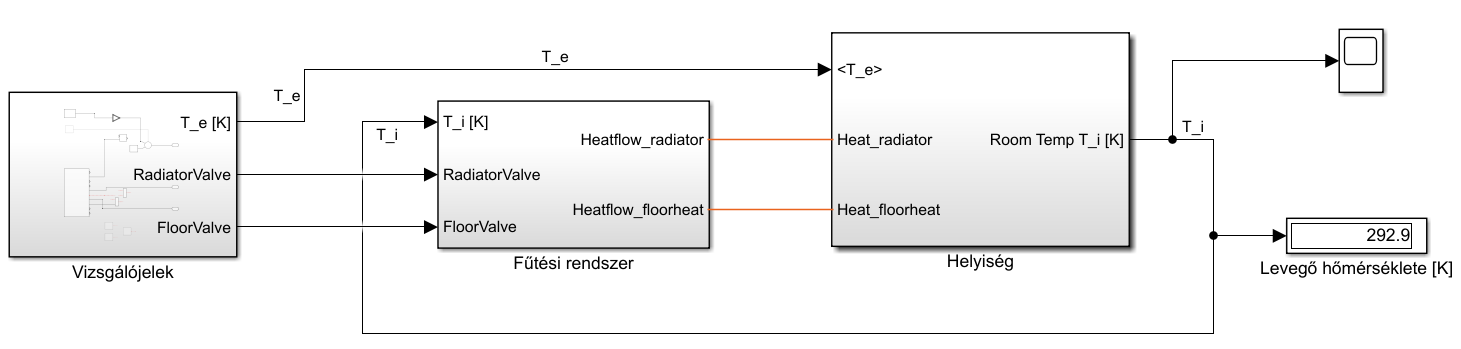
\includegraphics[trim=0 0 0 0, clip,width=\textwidth]{figures/simulink-network-minimalist-layout2}
	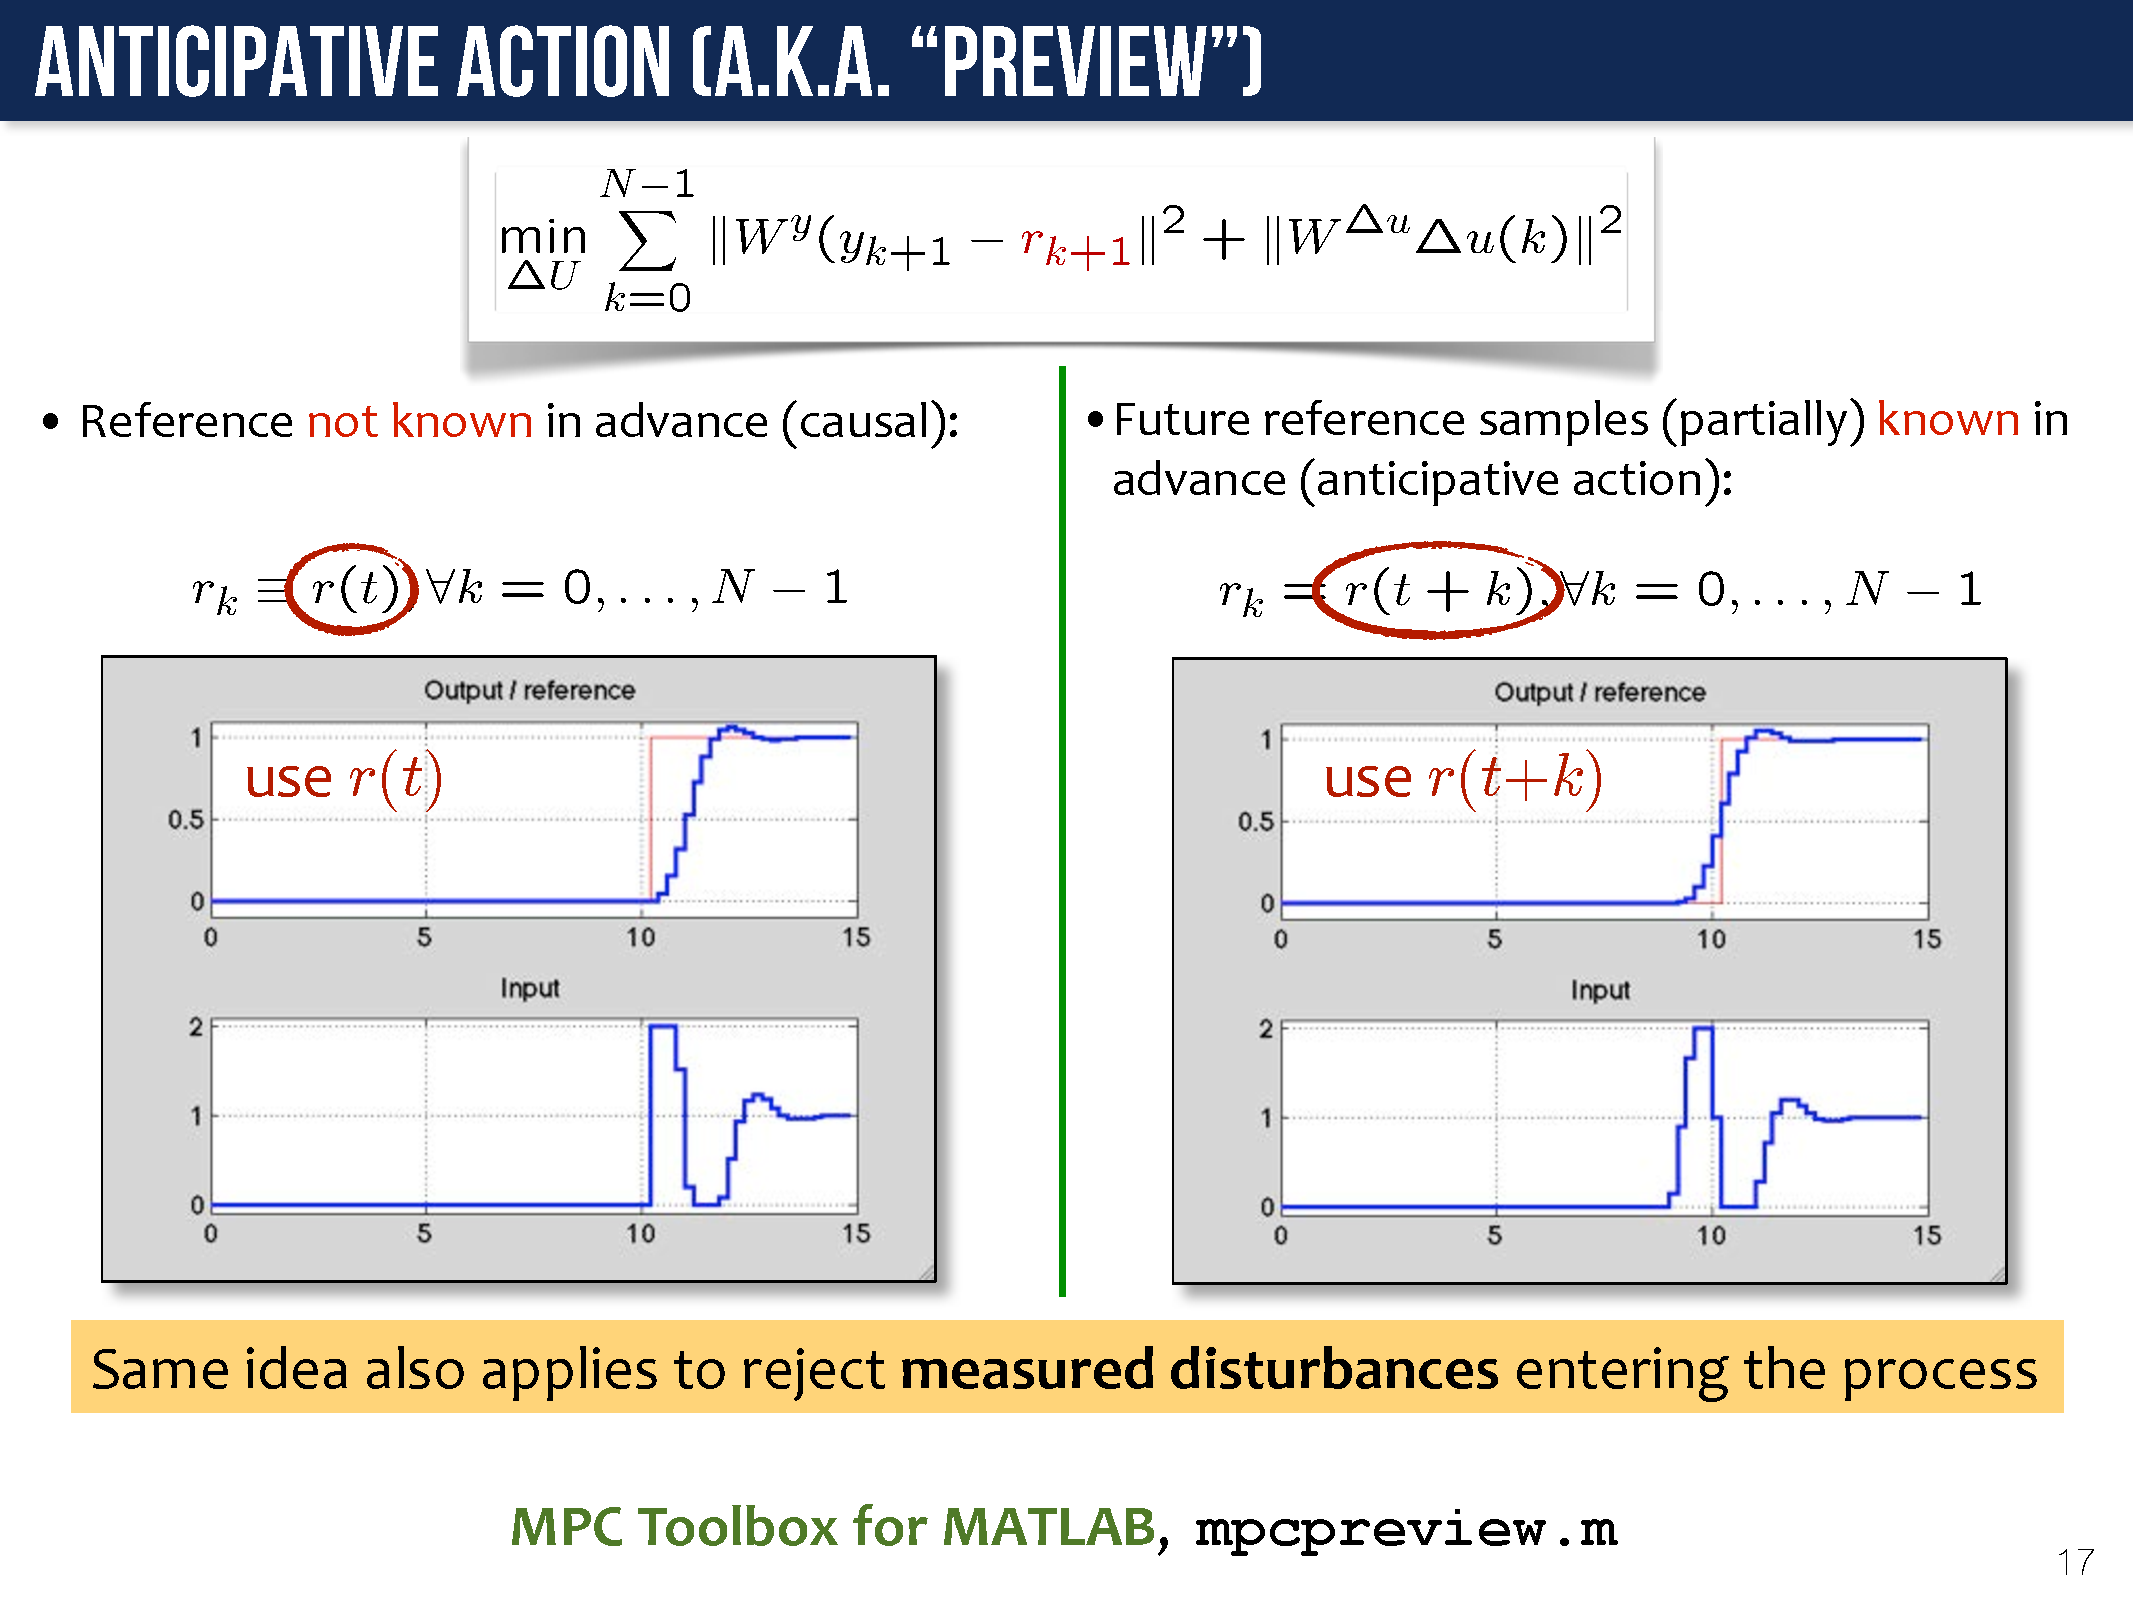
\includegraphics[trim=10 50 10 0, clip,width=\textwidth]{figures/onlab/preview}
	%\caption{Fűtési rendszer modellje - fűtőtest és helyiség}
	\label{fig:preview-bemporad}
\end{figure}

Erre abban az esetben van lehetőség, ha például elő van írva a napi hőmérséklet alapjel, ahogyan ez megtehető egyszerű programozható termosztátoknál is, amelyek egyszerű RBC (Rule Based Control) elven kapcsolnak be vagy ki.

Időjárás-előrejelzést figyelembe véve pedig a külső hőmérséklet értékére adható becslés, ami tovább csökkentheti az energiafelhasználást.

{\large 2) \underline{SÚLYOZÁS MÓDOSÍTÁSA} -- } A költségfüggvényben a beavatkozóknak különböző súlyokat rendelhetünk, ezzel szintén korlátozhatók a beavatkozó jelek. 

Még jobb eredményt lehet elérni időben változó súlyokat használva, ami például csúcsidőben magasabb energiaárakat elkerülve kiegyenlítheti a fogyasztást.
%
%
%\begin{figure}[H]
%	\centering
%	% trim={<left> <lower> <right> <upper>}
%	%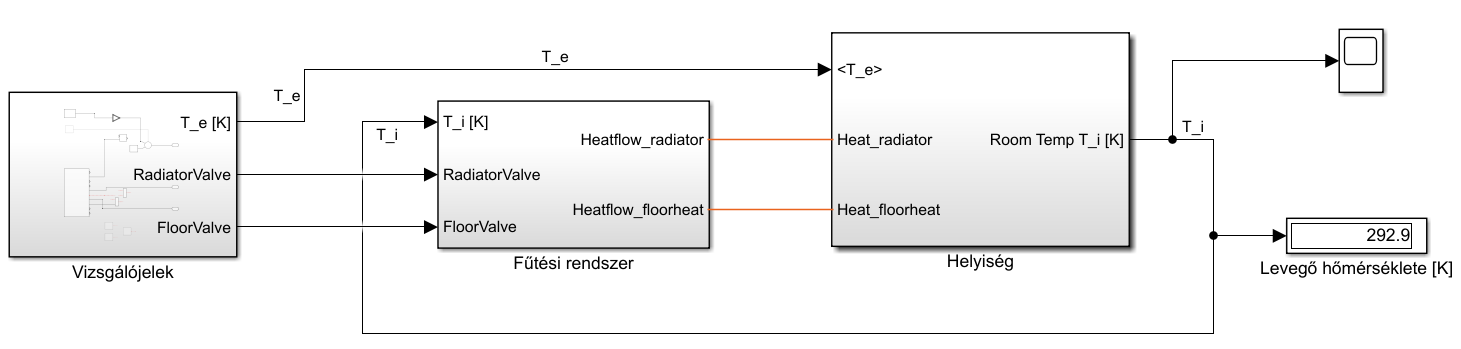
\includegraphics[trim=0 0 0 0, clip,width=\textwidth]{figures/simulink-network-minimalist-layout2}
%	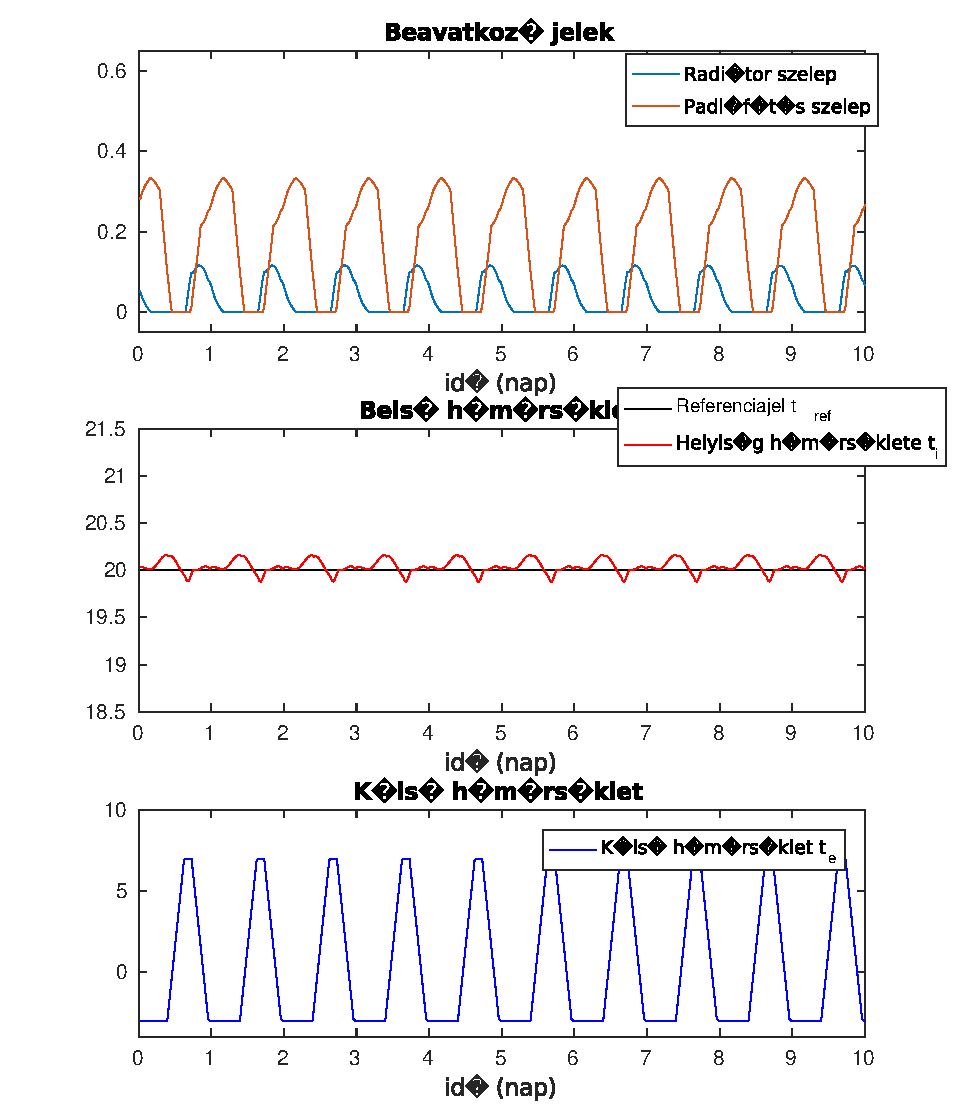
\includegraphics[trim=0 0 0 0, clip,width=0.4\textwidth]{figures/onlab/constRefPrev/Cconstref}
%	\caption{C szabályozó}
%	\label{fig:peak2-plottempC}
%\end{figure}
%
%
%\begin{figure}[H]
%	\centering
%	% trim={<left> <lower> <right> <upper>}
%	%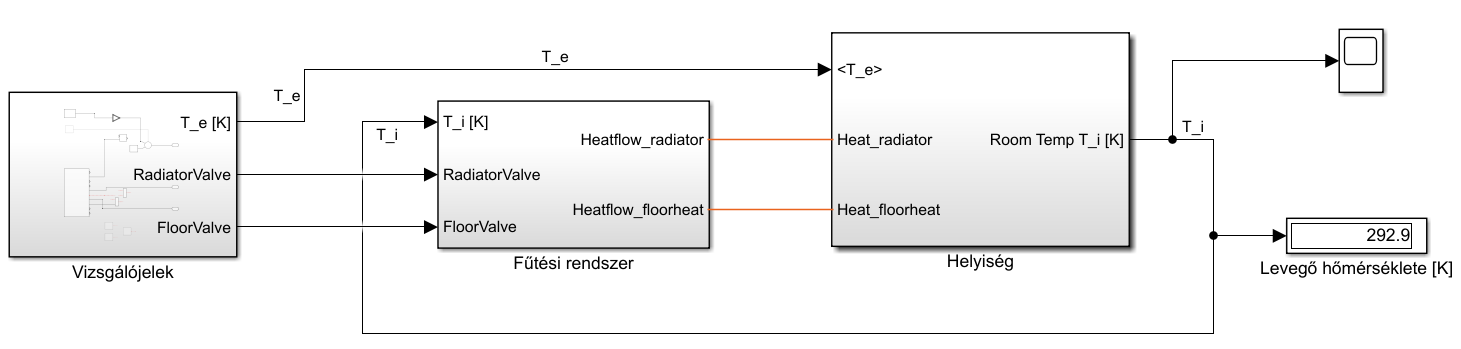
\includegraphics[trim=0 0 0 0, clip,width=\textwidth]{figures/simulink-network-minimalist-layout2}
%	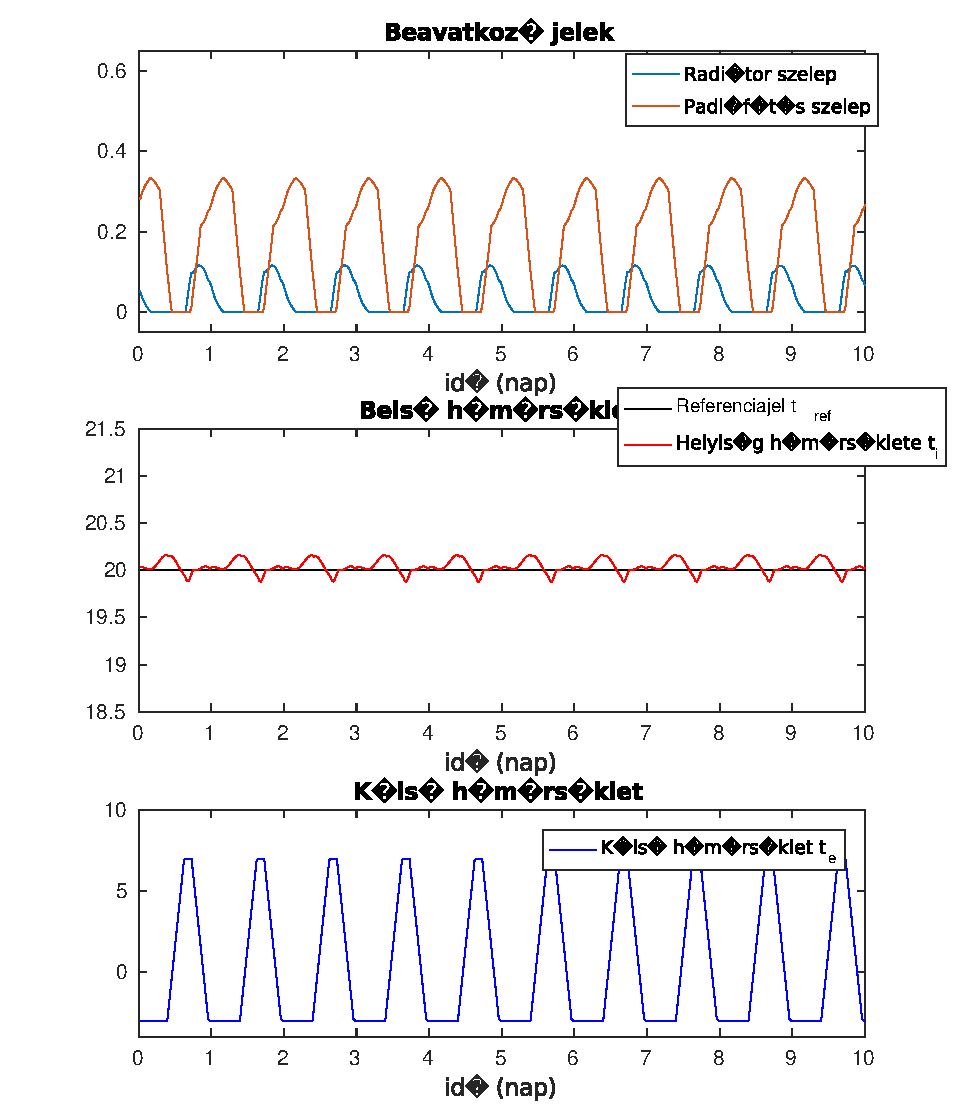
\includegraphics[trim=0 0 0 0, clip,width=0.4\textwidth]{figures/onlab/constRefPrev/Cconstref}
%	\caption{C szabályozó}
%	\label{fig:peak2-plottempC}
%\end{figure}


\begin{table}[H]
	\footnotesize
	\centering
	%\renewcommand{\arraystretch}{2} % to increase cell height
	%\taburulecolor{gray}
	%\begin{tabular}{|p{0.8cm}|p{1cm}|p{1cm}|p{1cm}|p{1cm}|p{1cm}|p{1cm}|p{1cm}|}
	%
	%\begin{tabulary}{\linewidth}{LLc}
	\begin{tabu}{@{}clll@{}}
		\hline
		$T_s$ 	& \multicolumn{3}{c}{30 perc}
		\\ 
		p & \multicolumn{3}{c}{48 óra}
		\\ 
		c 		& \multicolumn{3}{c}{1}
		\\ \hline
		szabályozó & C & C2 & C4
		\\
		
		$w_u$ 	& 0 & &
		\\ 
		$w_{\Delta u}$ 	& 50&&
		\\ 
		$w_y$ 	& 20&&
		\\
		SF 		& 30 &&
		\\   \hline
	\end{tabu}
	\label{tab:severalMPCweights}
	\caption{MPC szabályozó paraméterei}
	%
	%\label{tab:TabularExample}
	%\tabref{TabularExample}~táblázat
\end{table}


\begin{figure}[H]
	\begin{subfigure}[t]{0.32\textwidth}
		\centering
		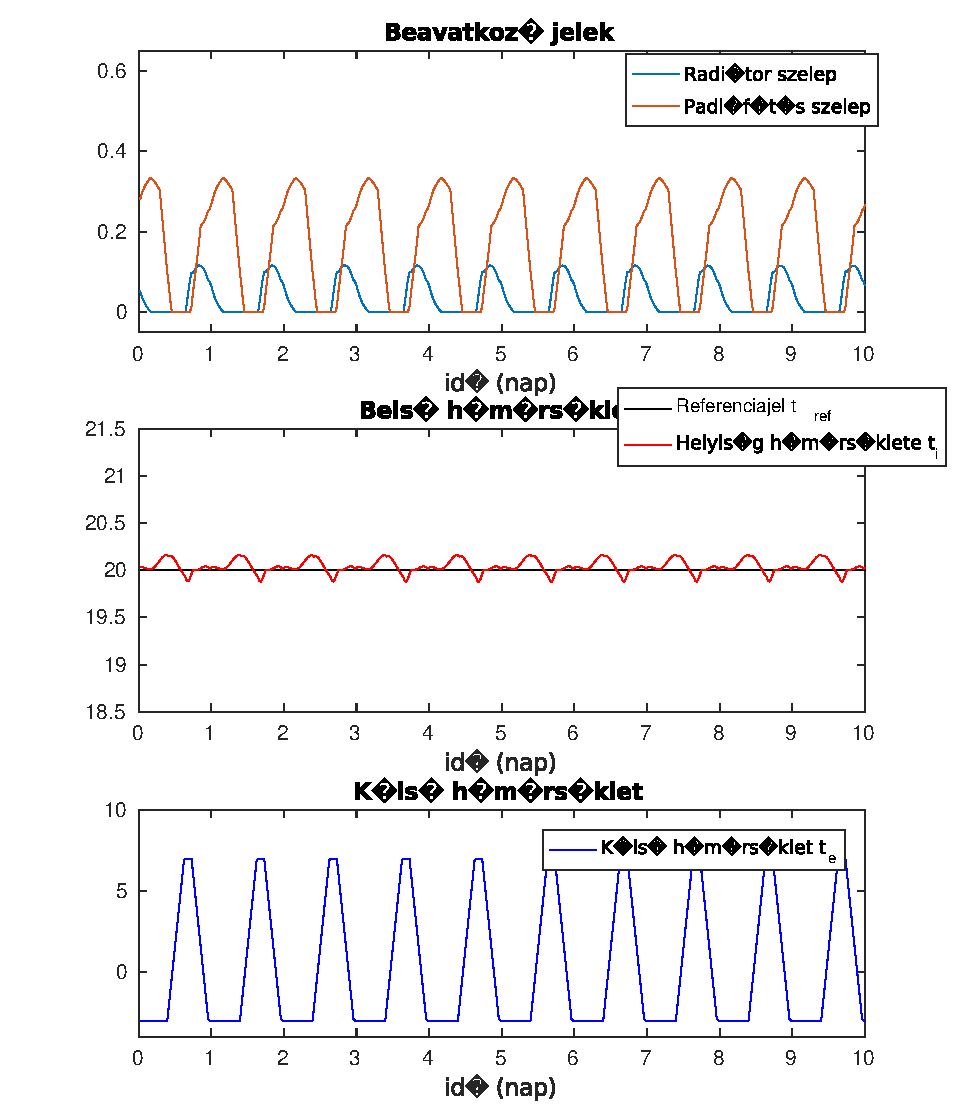
\includegraphics[trim=0 0 0 0, clip,width=\textwidth]{figures/onlab/constRefPrev/Cconstref}
		\caption{C szabályozó}
		\label{fig:constrefc}
	\end{subfigure}
	~
	\begin{subfigure}[t]{0.32\textwidth}
		\centering
		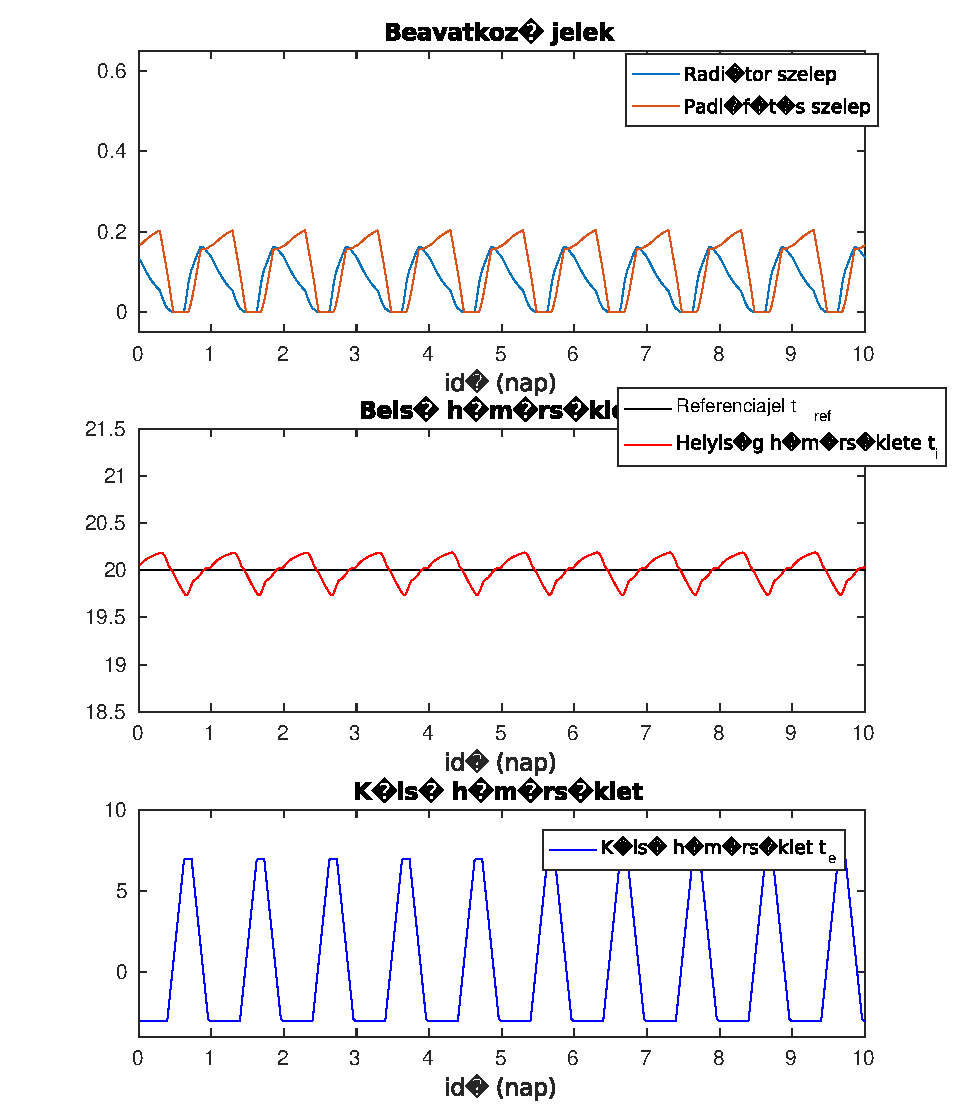
\includegraphics[trim=0 0 0 0, clip,width=\textwidth]{figures/onlab/constRefPrev/C2constref}
		\caption{C2 szabályozó}
		\label{fig:mpc-wy-2}
	\end{subfigure}
	~
	\begin{subfigure}[t]{0.32\textwidth}
		\centering
		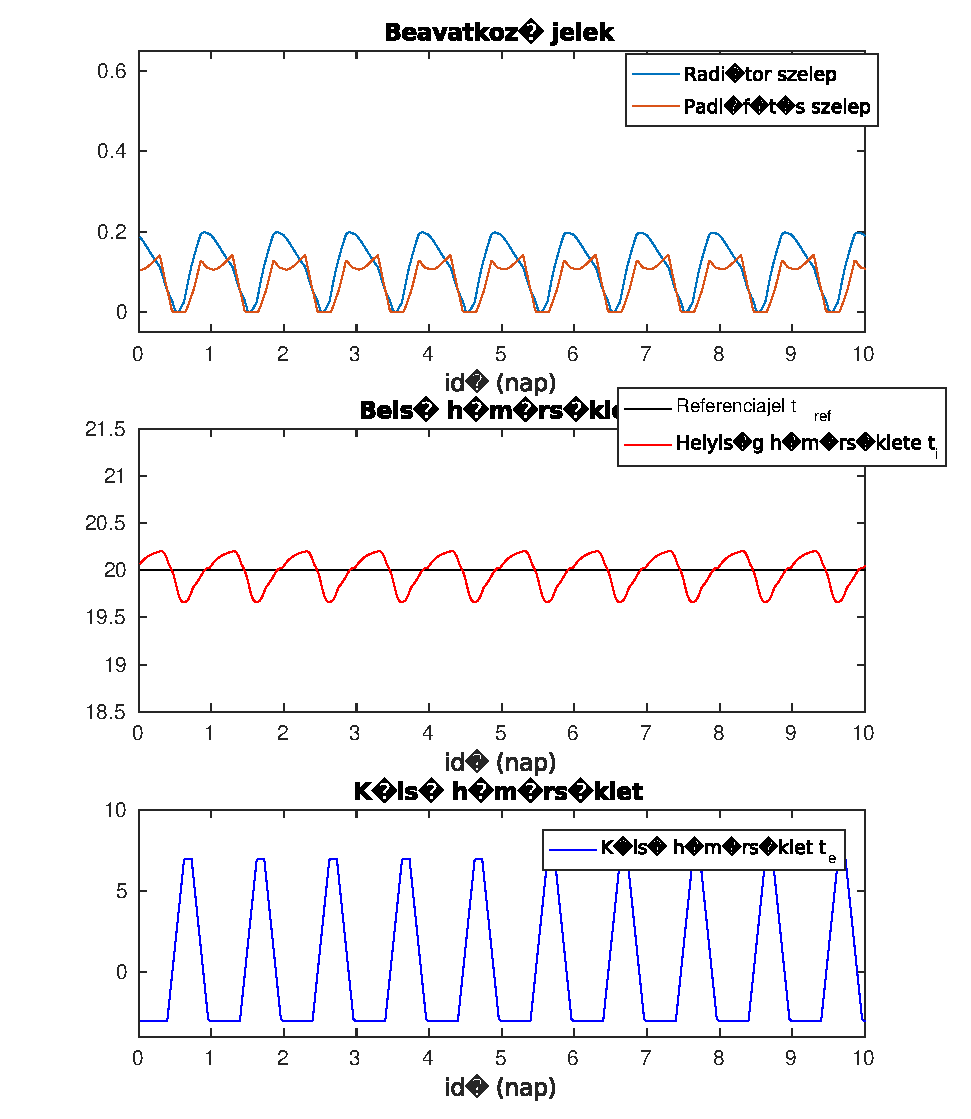
\includegraphics[trim=0 0 0 0, clip,width=\textwidth]{figures/onlab/constRefPrev/C4constref}
		\caption{C4 szabályozó}
		\label{fig:mpc-wy-5}
	\end{subfigure}
	\caption{MPC viselkedése -- previewing, kül. súlyokkal}
	\label{fig:mpc-previeWeight}
\end{figure}

A fentiekkel a szabályozók beavatkozóinak hőleadása:

Peak demandja:

\begin{figure}[H]
	%	% trim={<left> <lower> <right> <upper>}
	\begin{subfigure}[t]{0.48\textwidth}
		\centering
		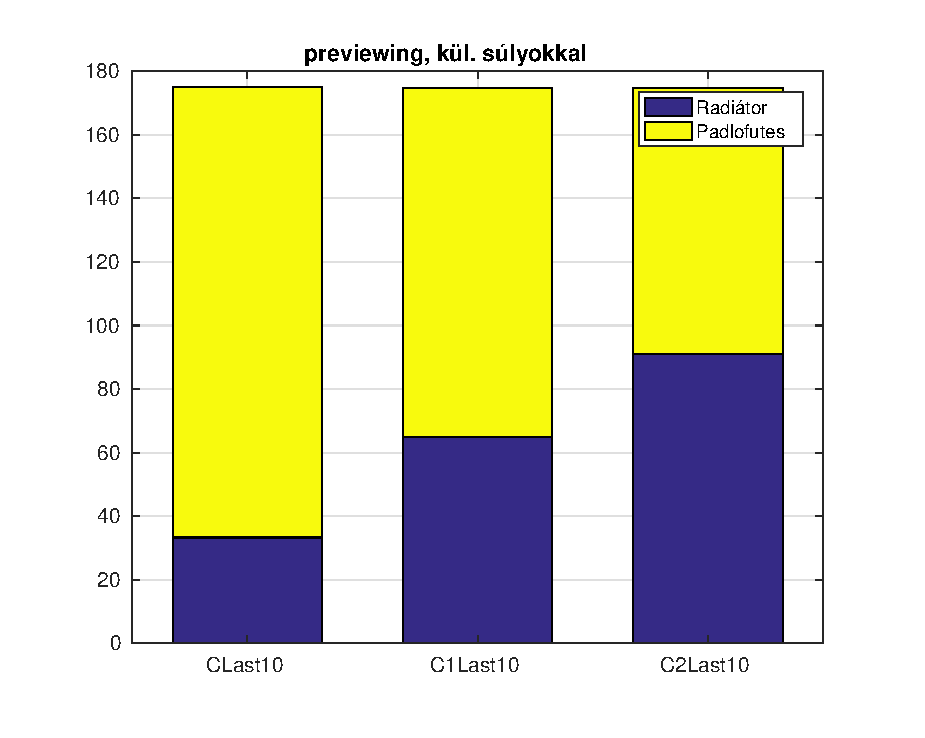
\includegraphics[trim=0 0 0 0, clip,width=1.1\textwidth]{figures/onlab/constRefPrev/summaryEnergy}
		\caption{Leadott homennyiseg megoszlasa}
		\label{fig:constrefHeat}
	\end{subfigure}
	~
	\begin{subfigure}[t]{0.48\textwidth}
		\centering
		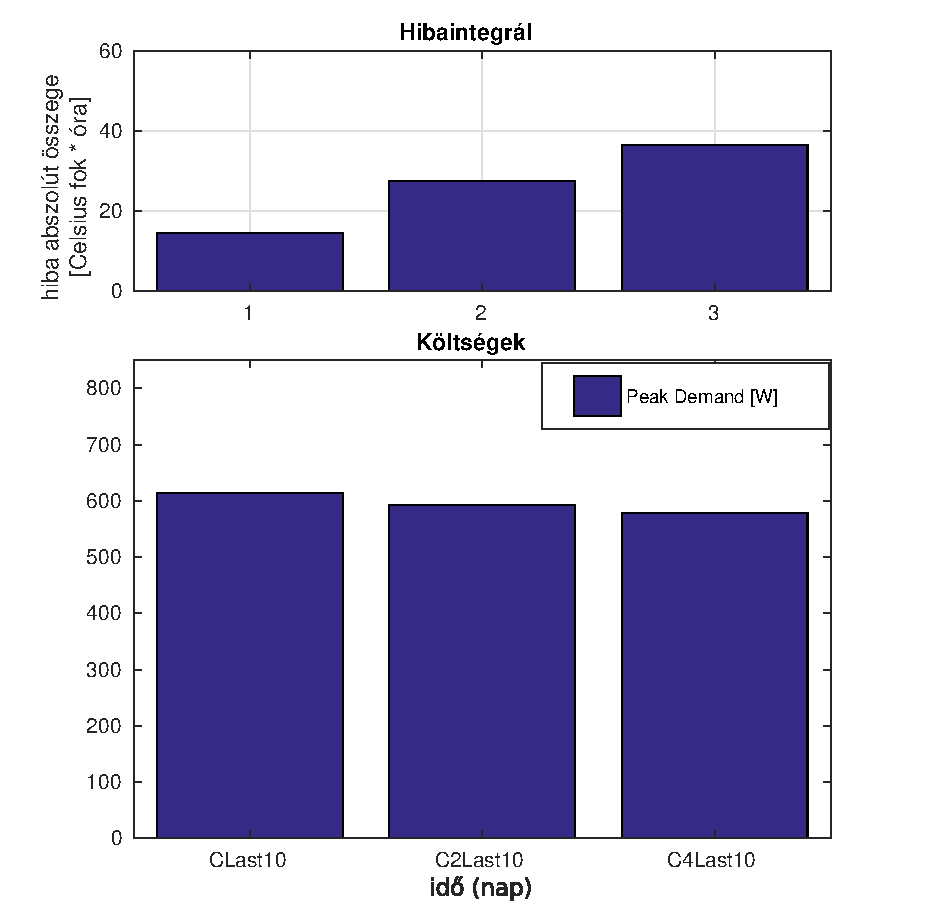
\includegraphics[trim=0 0 0 0, clip,width=1.1\textwidth]{figures/onlab/constRefPrev/summaryPeakDemand}
		\caption{C2 szabályozó}
		\label{fig:constrefPeak}
	\end{subfigure}
\end{figure}


\pagebreak

A munka során célul tűztem ki, hogy gyakorlatban használható, a felmerülő igényeket jobban kielégítő szabályozást állítsak fel.

Számos szempont merülhet fel,



A korábban identifikált lineáris modellt használtam fel



\begin{table}[H]
	\footnotesize
	\centering
	%\renewcommand{\arraystretch}{2} % to increase cell height
	%\taburulecolor{gray}
	%\begin{tabular}{|p{0.8cm}|p{1cm}|p{1cm}|p{1cm}|p{1cm}|p{1cm}|p{1cm}|p{1cm}|}
	%
	%\begin{tabulary}{\linewidth}{LLc}
	\begin{tabu}{@{}cl@{}}
		\hline
		$T_s$ 	& 1800 s
		\\ 
		p 		& 50 minta (25 óra)
		\\ 
		c 		& 1
		\\
		$w_u$ 	& 0.005 
		\\ 
		$w_{\Delta u}$ 	& 50
		\\ 
		$w_y$ 	& 20
		\\
		SF 		& 30 
		\\   \hline
	\end{tabu}
	\label{tab:severalMPCfactors}
	\caption{MPC szabályozó paraméterei}
	%
	%\label{tab:TabularExample}
	%\tabref{TabularExample}~táblázat
\end{table}


\section{Költségek figyelembe vétele}

A fűtés energiaköltségét legkönnyebben az összes felhasznált energia mennyiségéből kaphatjuk meg. Ezen kívül célszerű még megvizsgálni a maximális teljesítményigényt is (peak demand), illetve az energiaátalakítás teljesítményszintektől függő hatásfokát.

A csúcsidőszakban lecsökkent teljesítményigény különösen előnyös lehet akkor, ha a tarifák ebben az időszakban magasabbak.


A helyiség Simscape modelljéből ki lehetett vezetni a ténylegesen leadott hőmennyiséget, amiből már meg lehet állapítani a forintosított költségeket.


\section{Komfort figyelembe vétele}

A szabályozás ezen minőségi jellemzője a hibajellel arányos. Ennek átlaga egy referenciától mért átlagos eltérést ad, abszolút integrálva a hibát pedig kiválaszthatjuk a zavarokra minimális hibával működő szabályozást.

A szabványok igen széles tartományban adják meg a komfortos 

\subsection{Kritérium a szabályozásra}
Előírt tartományban kell a hőmérsékletnek maradnia (lásd szabvány ill. ETH Zürich).

\subsection{Hőérzetbeli különbségek}
Az időjárás-előrejelzések is megadnak hőérzetet a napsütés, szél függvényében.
Napos időben és szélcsendben melegebbnek tőnik az idő: hasonlóan kijelenthető, hogy sugárzó fűtések használatával a levegő hőmérséklete alacsonyabban is tartható ugyanakkora komfort eléréséhez.

Ezért célszerű $T_{AUST}$-t is megvizsgálni.

\section{Zavarelnyomás}

\section{Alapjel követése}

\subsection{Komfort -- Hibajel minimalizálása}
\subsection{Költség -- Beavatkozó jelek és a teljesítmény, peak demand}






